\chapter{Implementation}
\label{impl}

This chapter presents the implementation and architecture of this stereo vision system.

\section{Architecture Overview}

The stereo vision system module in this paper is composed of three main parts: SADs, minimum comparators, and a wrapper around the previous two that takes in image data and outputs disparity values.

The code for the following sections is located on github under:
\\\path{https://github.com/cccitron/mastersThesis}.

\subsection{Sum of the Absolute Differences Architecture}

Two versions of the SAD algorithm have been implemented in this paper. The first uses a 9x9 window and the other one uses a 7x7 window. Figure~\ref{fig:sadAlg_rtl} shows the top level entity of how the SAD implementation used. Both versions have a clocked input (clk\_I) and a one bit data input (data\_I) to notify the algorithm to begin calculating the SAD value. The tempalte\_window\_I and search\_window\_I between the two versions differ in the sense that the number of bytes, 49 or 81, sent to the sadAlgorithm entity are different. The data\_O signals when the calculation is complete and ready that the algorithm is ready for the next set of input. The calculated SAD value is sent out of the entity through sad\_O.

There is a slight variation between the standard SAD algorithm and how it is implemented in this stereo vision system. Instead of subtracting two pixel values and then taking the absolute difference between them, the implementation in this paper first finds which corresponding pixel has a greater value and then sends the two pixels to the subtracter based on that. See APPENDIX (INSERT NEEDED) for the code used. The subtracter then takes the greater value and subtracts from it the lesser value and returns the difference. This difference, since it will always be greater than or equal to zero, will always be equal to the absolute difference of the two corresponding pixels. This process was implemented to reduce the complexity of using signed values and allowed for the number of bytes used for logic in the algorithm to be reduced by one bit.

\begin{figure}[h]
	\begin{center}
		\includegraphics[width=100mm]{figures/sadAlgorithm_rtl.png}
		\captionfonts
		\caption{The top level SAD algorithm implementation.}
		\label{fig:sadAlg_rtl}
	\end{center}
\end{figure}


\subsubsection{State Diagram}

Inside the sadAlgorithm entity from Fig.~\ref{fig:sadAlg_rtl}, the state machine from Figure~\ref{fig:stateMachine} controls the SAD algorithm. The state machine begins at SO and initializes all the values used in it to 0. It then proceeds to S1 where the state machine remains on standby until data\_I becomes '1'. In S2, the counter begins from 0, the subtraction between respective pixel values begins, and on the next clock cycle, the state will be S3. While in S3, the counter is incremented by 1 every clock cycle. S3 is where the SAD algorithm is performed. After the counter is equal to windowSize (7 for the 7x7 and 81 for the 9x9, see the sections below for details), the SAD calculation is complete. The state machine sets data\_O to 1 to notify the SAD wrapper that the calculation is complete and it then moves to S1 and waits for new input.

\begin{figure}[h]
	\begin{center}
		\includegraphics[width=100mm]{figures/stateMachine.png}
		\captionfonts
		\caption{The state machine for implementing the SAD algorithm.}
		\label{fig:stateMachine}
	\end{center}
\end{figure}


\subsubsection{9x9 Window}
\label{sec:9x9window}

The 9x9 window implementation operated with 4 pixels being processed in parallel to get their disparity values. Each pixel has 16 SAD operations occurring in parallel. With 64 SAD operations happening in parallel, each SAD calculation needed to process their windows with a higher degree of serialization in order to reduce space to fit on the Atlys board ~\cite{atlysBoard}. Figure~\ref{fig:sadAlg9x9} shows a simplified version of this process. Each clock cycle, for 81 cycles, the difference between corresponding pixels is calculated. Beginning one clock cycle after the differences begin to be calculated, so there is a value, sub, to use. The sum\_out is added to itself and sub. This process also occurs 81 times, one addition each clock cycle. Every clock cycle, a new \"absolute\" difference value is added to the sum\_out. The state machine in Fig.~\ref{fig:stateMachine} stops the calculation for sum\_out after the full SAD value has been summed up.

\begin{figure}[h]
	\begin{center}
		\includegraphics[width=120mm]{figures/sadAlgorithm9x9.png}
		\captionfonts
		\caption{Architecture overview of the SAD algorithm with the 9x9 window implementation.}
		\label{fig:sadAlg9x9}
	\end{center}
\end{figure}

Figure~\ref{fig:sadPipe9x9} illustrates the pipeline used for the 9x9 window version. It takes 81 clock cycles to take all of the differences between all 81 pairs of pixel values. After the first difference is calculated, the differences can then begin to be summed up. The summing also takes 81 clock cycles and ends one cycle after the last difference is calculated. This results in a time of 82 clock cycles.

\begin{figure}[h]
	\begin{center}
		\includegraphics[width=60mm]{figures/sadPipeline9x9.png}
		\captionfonts
		\caption{Pipeline architecture of the SAD algorithm with the 9x9 window implementation.}
		\label{fig:sadPipe9x9}
	\end{center}
\end{figure}

The code for the 9x9 window implementation can be found on github:
\\\path{https://github.com/cccitron/mastersThesis/tree/master/makestuff/libs/libfpgalink-20120621/hdl/fx2/vhdl/sad_simple_reg_9x9/}

\subsubsection{7x7 Window}

The 7x7 window implementation operated with 2 pixels being processed in parallel to get their disparity values. Each pixel has 16 SAD operations occurring in parallel. With only 32 SAD operations happening in parallel, as opposed to 64 that were done in parallel in Section~\ref{sec:9x9window} and with a window size that has used 32 pixels for each window in each SAD calculation, the process could utilize a higher degree of parallelization.

\begin{figure}[h]
	\begin{center}
		\includegraphics[width=120mm]{figures/sadAlgorithm7x7.png}
		\captionfonts
		\caption{Architecture overview of the SAD algorithm with the 7x7 window implementation.}
		\label{fig:sadAlg7x7}
	\end{center}
\end{figure}


\begin{figure}[h]
	\begin{center}
		\includegraphics[width=60mm]{figures/sadPipeline7x7.png}
		\captionfonts
		\caption{Pipeline architecture of the SAD algorithm with the 7x7 window implementation.}
		\label{fig:sadPipe7x7}
	\end{center}
\end{figure}


\subsection{Minimum Comparator Architecture}


\begin{figure}[h]
	\begin{center}
		\includegraphics[width=100mm]{figures/minComparator_rtl.png}
		\captionfonts
		\caption{The top level minimum comparator implementation.}
		\label{fig:minComp_rtl}
	\end{center}
\end{figure}


\begin{figure}[h]
	\begin{center}
		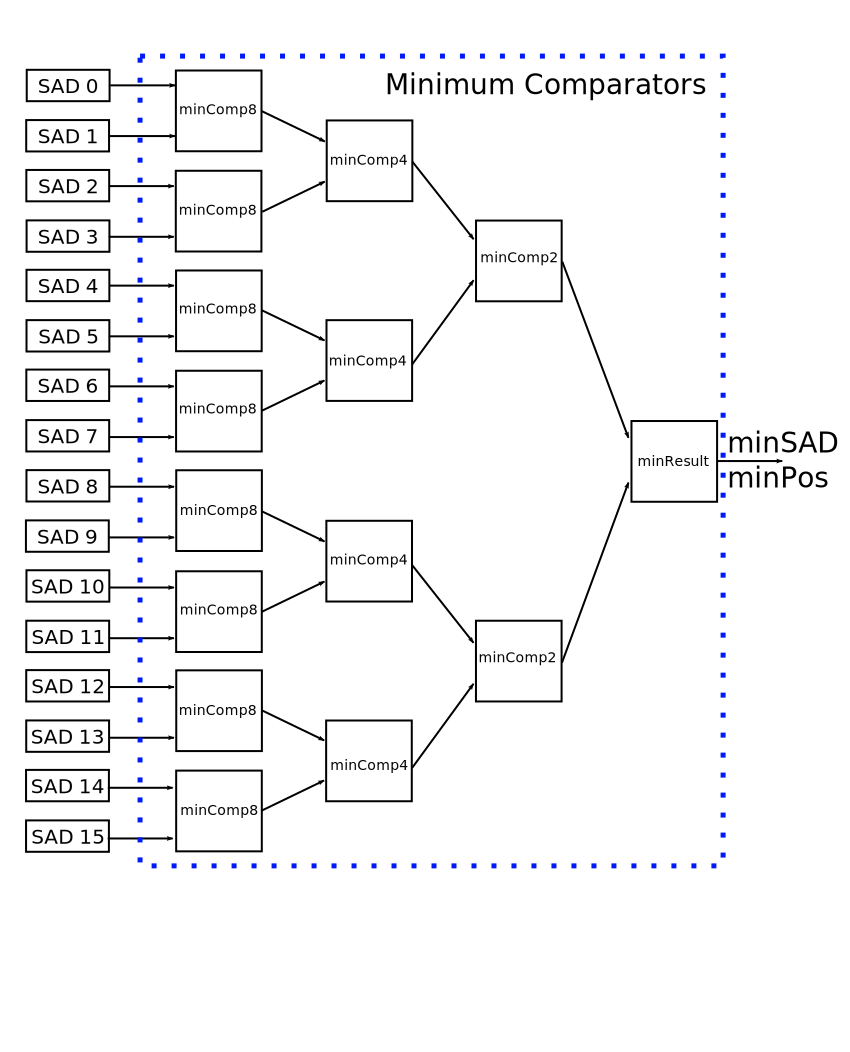
\includegraphics[width=150mm]{figures/minComparator.png}
		\captionfonts
		\caption{The minimum comparator tree designed to quickly find the minimum value and corresponding index out of the 16 SAD values that are calculated for one pixel.}
		\label{fig:minComp}
	\end{center}
\end{figure}


\subsection{SAD Wrapper}

\begin{figure}[h]
	\begin{center}
		\includegraphics[width=100mm]{figures/sad_wrapper_rtl.png}
		\captionfonts
		\caption{The SAD wrapper that encompasses the SAD algorithm and minimum comparator. It interacts with the top level.}
		\label{fig:sadWrapper_rtl}
	\end{center}
\end{figure}


\subsection{Top Level}

\begin{figure}[h]
	\begin{center}
		\includegraphics[width=150mm]{figures/top_level_rtl.png}
		\captionfonts
		\caption{The overview of the structure used for implementing the 9x9 window. The 7x7 window has two less SAD and minComp each.}
		\label{fig:topLevel_rtl}
	\end{center}
\end{figure}

\section{FPGA and Computer Communication}



\subsection{FPGALink}



